\section{Real World Experiments} \label{app:real}

We create a real-world version of \textbf{Trampoline} dataset for use in our sim to real experiments.
To mimic the simulated scene, solid balls of various materials and densities (see Table \ref{tab:real_spheres}) are dropped into rubber sheets of various thicknesses (see Table \ref{tab:real_sheets}).
The balls are dropped using a Franka Emika Panda robot, where the in-plane drop position is sampled from a volume of \SI{4}{\cm} x \SI{4}{\cm} x \SI{5}{\cm}.
The scene is recorded using a StereoLabs Zed Mini stereo camera at a resolution of $720$x$1280$ frame rate of \SI{30}{fps}.

\begin{table}[ht]
\centering
\begin{tabular}{c c l}
\toprule
\textbf{Diameter} (\si{\mm}) & \textbf{Mass} (\si{\g}) & \textbf{Material} \\
\midrule
40 & 269 & Steel Solid \\
40 & 69  & Steel Hollow \\
50 & 110 & Steel Hollow \\
60 & 162 & Steel Hollow \\
40 & 21  & PLA 50\% Infill \\
\bottomrule
\end{tabular}
\vspace{0.1cm}
\caption{Sphere specifications used in the real-world experiments.}
\label{tab:real_spheres}
\end{table}

\begin{table}[ht]
\centering
\begin{tabular}{l c c}
\toprule
\textbf{Color} & \textbf{Thickness} (\si{\mm}) & \textbf{Average Density} (\si{\kg\per\m\cubed}) \\
\midrule
Black  & 0.381  & 992.7 \\
Green  & 0.254  & 992.7 \\
Yellow & 0.1524 & 992.7 \\
\bottomrule
\end{tabular}
\vspace{0.1cm}
\caption{Sheet specifications used in the real-world experiments.}
\label{tab:real_sheets}
\end{table}

Depth estimates for each recorded frame are recomputed using FoundationStereo~\citep{FoundationStereo} (smaller architecture based on Vit-small).
Images are resized to $480$x$853$ and are converted into point clouds by unprojecting the depth using the cameras' intrinsic parameters.
The camera extrinsics are calibrated by mounting Aruco markers on the frame around the rubber sheet and optimizing for minimal reprojection error (OpenCV's \texttt{solvePnPRansac}).
Point clouds are then transformed into a canonical world frame such that the bottom left corner of the sheet is at the origin and the sheet is on the xy plane.

We discard time steps before the ball begins to fall and limit trajectories to 20 time steps (approx. \SI{0.667}{\s}).
Points in the background of the scene are cropped out, and voxel downsampling is applied with a voxel edge length of \SI{5}{\mm}.
To remove spurious artifacts, any points that have fewer than $20$ neighbours within a radius of \SI{15}{\mm} are filtered out.
Finally, \gls{fps}~\citep{ruizhongtai2017pointnet} is applied to reduce the point clouds to 2048 points.

Sphere points are identified via color segmentation, isolating the distinctly colored ball from the scene.
The color labels are refined through an iterative algorithm that updates each point's label based on its own color and the colors of its neighbors, smoothing spurious misclassifications at object boundaries.
Given the known sphere diameter, a spherical mask is fitted to the identified sphere points by optimizing the center position, which is then used to remove robot arm points that fall outside the mask.
Finally, \gls{fps} is applied to reduce the point clouds to 1024 points.


\subsection{Robustness to Corrupted Observations}
\label{app:corruption}

Real-world point clouds can contain missing regions, for example due to occlusions or reflective surfaces, as well as spurious points from reconstruction errors. To evaluate how robust \gls{peach} is to such artifacts, we corrupt the context observations of the real-world \texttt{Trampoline} scene at test time.

\paragraph{Setup.}
We use the \gls{peach} model from the main experiments, as well as a \gls{peach} model trained with the identical setup but without data augmentation. For each corruption level, we remove $1\%$, $9\%$, or $25\%$ of the points of each context point cloud, which we refer to as low, medium, and high corruption. Instead of removing points uniformly at random, we remove them in small spatially connected patches, which resembles missing regions in real sensor data. We additionally insert the same number of spurious points at random locations in the scene to simulate reconstruction artifacts. Only the context trajectories are corrupted. The encoder infers the latent material description from the corrupted context, and the simulator predicts the target trajectory from it. We evaluate this prediction against the uncorrupted observations of the target trajectory using the same point-to-mesh distance as in Figure~\ref{fig:qualitative_realworld}. Note that these corruptions are similar in kind to the region dropout and point artifacts used in our data augmentation, but they are applied to real-world instead of simulated observations and at levels that we did not tune for this evaluation.

\paragraph{Results.}
Figure~\ref{fig:corruption} shows the results. \gls{peach} handles all three corruption levels similarly well, and its errors remain close to the uncorrupted case throughout the trajectory. Even under high corruption, \gls{peach} is clearly more accurate than the \textit{Oracle} during the contact phase, although the \textit{Oracle} does not rely on the context observations and is therefore unaffected by the corruption. In contrast, the \gls{peach} model trained without data augmentation deteriorates considerably under high corruption, and its error at the peak of the contact phase approaches that of the \textit{No Context} baseline. This shows that data augmentation is essential for the robustness of \gls{peach} to corrupted real-world observations.

\begin{figure}[t]
    \centering
    \makebox[\textwidth][c]{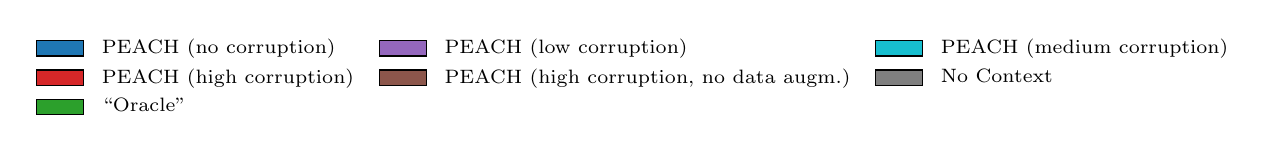
\begin{tikzpicture}
    \tikzstyle{every node}=[font=\scriptsize]
    \definecolor{tabblue}{RGB}{31, 119, 180}
\definecolor{taborange}{RGB}{255, 127, 14}
\definecolor{tabgreen}{RGB}{44, 160, 44}
\definecolor{tabred}{RGB}{214, 39, 40}
\definecolor{tabpurple}{RGB}{148, 103, 189}
\definecolor{tabbrown}{RGB}{140, 86, 75}
\definecolor{tabpink}{RGB}{227, 119, 194}
\definecolor{tabgray}{RGB}{127, 127, 127}
\definecolor{tabolive}{RGB}{188, 189, 34}
\definecolor{tabcyan}{RGB}{23, 190, 207}
\definecolor{ForestGreen}{RGB}{34, 139, 34}

    \begin{axis}[%
        hide axis,
        xmin=10,
        xmax=50,
        ymin=0,
        ymax=0.1,
        legend style={
            draw=none,
            legend cell align=left,
            legend columns=3,
            /tikz/every odd column/.append style={column sep=1ex},
            /tikz/every even column/.append style={column sep=1.6ex},
        }
    ]

        \addlegendimage{area legend, fill=tabblue}
    \addlegendentry{PEACH (no corruption)}

    \addlegendimage{area legend, fill=tabpurple}
    \addlegendentry{PEACH (low corruption)}

    \addlegendimage{area legend, fill=tabcyan}
    \addlegendentry{PEACH (medium corruption)}

    \addlegendimage{area legend, fill=tabred}
    \addlegendentry{PEACH (high corruption)}

        \addlegendimage{area legend, fill=tabbrown}
    \addlegendentry{PEACH (high corruption, no data augm.)}

    \addlegendimage{area legend, fill=tabgray}
    \addlegendentry{No Context}

    \addlegendimage{area legend, fill=tabgreen}
    \addlegendentry{``Oracle''}

    \end{axis}
\end{tikzpicture}}\\[-2mm]
    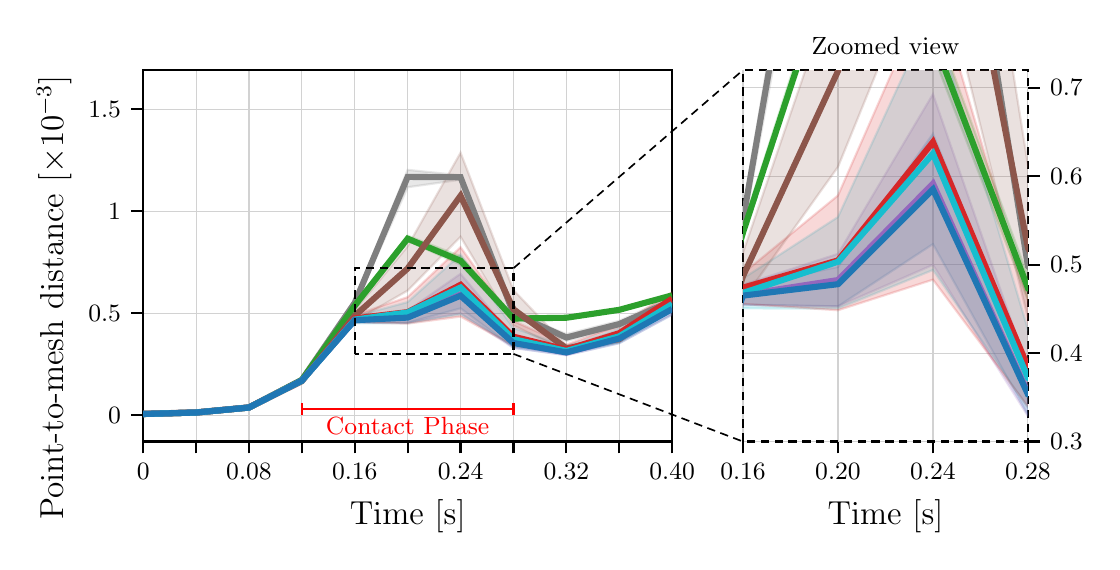
\begin{tikzpicture}

\definecolor{crimson2143940}{RGB}{214,39,40}
\definecolor{forestgreen4416044}{RGB}{44,160,44}
\definecolor{darkturquoise23190207}{RGB}{23,190,207}
\definecolor{gray127}{RGB}{127,127,127}
\definecolor{lightgray204}{RGB}{204,204,204}
\definecolor{mediumpurple148103189}{RGB}{148,103,189}
\definecolor{sienna1408675}{RGB}{140,86,75}
\definecolor{steelblue31119180}{RGB}{31,119,180}

% Plot content, shared by the full view and the zoomed view
\newcommand{\ablationcontent}{%
% Shaded areas
% No Context
\path [draw=gray127, fill=gray127, opacity=0.18]
(axis cs:0,8.07295291394894e-06)
--(axis cs:0,5.12359331139578e-06)
--(axis cs:1,1.24465407043317e-05)
--(axis cs:2,3.70405652006411e-05)
--(axis cs:3,0.000170184562616669)
--(axis cs:4,0.000538726298991605)
--(axis cs:5,0.00111711371160709)
--(axis cs:6,0.0011539952494968)
--(axis cs:7,0.000493944165682478)
--(axis cs:8,0.000363235438599077)
--(axis cs:9,0.000430213335330336)
--(axis cs:10,0.000541865832110489)
--(axis cs:10,0.000579285589992651)
--(axis cs:10,0.000579285589992651)
--(axis cs:9,0.000462110629396193)
--(axis cs:8,0.000397154613974635)
--(axis cs:7,0.000502686903510039)
--(axis cs:6,0.00117566139379051)
--(axis cs:5,0.00120230794382223)
--(axis cs:4,0.000562686173348084)
--(axis cs:3,0.000175566404236633)
--(axis cs:2,3.94724731199858e-05)
--(axis cs:1,1.48931526597096e-05)
--(axis cs:0,8.07295291394894e-06)
--cycle;
% Oracle
\path [draw=forestgreen4416044, fill=forestgreen4416044, opacity=0.18]
(axis cs:0,5.02822931252922e-06)
--(axis cs:0,5.00629528346508e-06)
--(axis cs:1,1.22442673364276e-05)
--(axis cs:2,3.64980695599115e-05)
--(axis cs:3,0.000170152035236697)
--(axis cs:4,0.000531509038712556)
--(axis cs:5,0.000854251318701245)
--(axis cs:6,0.000737646454490459)
--(axis cs:7,0.00045989315263796)
--(axis cs:8,0.000471600066430256)
--(axis cs:9,0.000512676674770773)
--(axis cs:10,0.000583336630952544)
--(axis cs:10,0.00059101728056703)
--(axis cs:10,0.00059101728056703)
--(axis cs:9,0.000520028840073792)
--(axis cs:8,0.000481395700517169)
--(axis cs:7,0.00048684069643059)
--(axis cs:6,0.000778906577484122)
--(axis cs:5,0.000879407519557844)
--(axis cs:4,0.000544052049326638)
--(axis cs:3,0.000173569310650237)
--(axis cs:2,3.67153696726064e-05)
--(axis cs:1,1.23036071607885e-05)
--(axis cs:0,5.02822931252922e-06)
--cycle;
% PEACH, no data corruption
\path [draw=steelblue31119180, fill=steelblue31119180, opacity=0.18]
(axis cs:0,5.32954746347514e-06)
--(axis cs:0,5.02559393680713e-06)
--(axis cs:1,1.23165469415198e-05)
--(axis cs:2,3.64593142171543e-05)
--(axis cs:3,0.000166523760070731)
--(axis cs:4,0.000454926606626032)
--(axis cs:5,0.000452832707678681)
--(axis cs:6,0.000523227875182783)
--(axis cs:7,0.000330028291073177)
--(axis cs:8,0.00029419582178889)
--(axis cs:9,0.000352838265921491)
--(axis cs:10,0.000491633596502652)
--(axis cs:10,0.000551979309175294)
--(axis cs:10,0.000551979309175294)
--(axis cs:9,0.000401096724481249)
--(axis cs:8,0.000327221116303917)
--(axis cs:7,0.000380109390453072)
--(axis cs:6,0.000648042633774821)
--(axis cs:5,0.000497473443410854)
--(axis cs:4,0.000475108261580317)
--(axis cs:3,0.000171479885157169)
--(axis cs:2,3.71906361107221e-05)
--(axis cs:1,1.26398031545705e-05)
--(axis cs:0,5.32954746347514e-06)
--cycle;
% PEACH, low corruption
\path [draw=mediumpurple148103189, fill=mediumpurple148103189, opacity=0.18]
(axis cs:0,5.33181615367084e-06)
--(axis cs:0,5.02817173014591e-06)
--(axis cs:1,1.22632851156368e-05)
--(axis cs:2,3.66258090542715e-05)
--(axis cs:3,0.000166674461158891)
--(axis cs:4,0.000454452977733126)
--(axis cs:5,0.000452836301428761)
--(axis cs:6,0.000499798321070557)
--(axis cs:7,0.000328714824713643)
--(axis cs:8,0.00029355594457229)
--(axis cs:9,0.000352027315361738)
--(axis cs:10,0.000493364606927571)
--(axis cs:10,0.000555784692805901)
--(axis cs:10,0.000555784692805901)
--(axis cs:9,0.000406913539591187)
--(axis cs:8,0.000328428077164062)
--(axis cs:7,0.000381828197077994)
--(axis cs:6,0.00069285897433474)
--(axis cs:5,0.000512243240027601)
--(axis cs:4,0.000477392968850836)
--(axis cs:3,0.000170880966390996)
--(axis cs:2,3.73897589736316e-05)
--(axis cs:1,1.2591421818513e-05)
--(axis cs:0,5.33181615367084e-06)
--cycle;
% PEACH, medium corruption
\path [draw=darkturquoise23190207, fill=darkturquoise23190207, opacity=0.18]
(axis cs:0,5.33187008670666e-06)
--(axis cs:0,5.02004117947763e-06)
--(axis cs:1,1.22499115414598e-05)
--(axis cs:2,3.66078880614396e-05)
--(axis cs:3,0.000166816796038916)
--(axis cs:4,0.000450620220369728)
--(axis cs:5,0.000450336349194913)
--(axis cs:6,0.000493966865518587)
--(axis cs:7,0.000338240592082002)
--(axis cs:8,0.000302442142137807)
--(axis cs:9,0.000356318301228384)
--(axis cs:10,0.000509605018251023)
--(axis cs:10,0.000578903033492679)
--(axis cs:10,0.000578903033492679)
--(axis cs:9,0.000422849455881078)
--(axis cs:8,0.000337414472119235)
--(axis cs:7,0.000426695050123271)
--(axis cs:6,0.000786849888509096)
--(axis cs:5,0.000553860430336499)
--(axis cs:4,0.000484498826608615)
--(axis cs:3,0.000170086979523234)
--(axis cs:2,3.72754672028037e-05)
--(axis cs:1,1.25844655204332e-05)
--(axis cs:0,5.33187008670666e-06)
--cycle;
% PEACH, high corruption
\path [draw=crimson2143940, fill=crimson2143940, opacity=0.18]
(axis cs:0,5.34417178130297e-06)
--(axis cs:0,5.01722694821183e-06)
--(axis cs:1,1.22452144020713e-05)
--(axis cs:2,3.66340591415337e-05)
--(axis cs:3,0.000167807462109977)
--(axis cs:4,0.000455630003959868)
--(axis cs:5,0.000448458030350594)
--(axis cs:6,0.000483019394023358)
--(axis cs:7,0.000339448086815537)
--(axis cs:8,0.000306087640065016)
--(axis cs:9,0.000377171187386921)
--(axis cs:10,0.000540727655061346)
--(axis cs:10,0.000602633721396614)
--(axis cs:10,0.000602633721396614)
--(axis cs:9,0.000439884008565059)
--(axis cs:8,0.000345229242002461)
--(axis cs:7,0.000460848601351245)
--(axis cs:6,0.000823033929511894)
--(axis cs:5,0.000578241476969197)
--(axis cs:4,0.000490163438494164)
--(axis cs:3,0.000170229076906026)
--(axis cs:2,3.73482912800682e-05)
--(axis cs:1,1.25838650814103e-05)
--(axis cs:0,5.34417178130297e-06)
--cycle;
% PEACH, high corruption, no data augmentation
\path [draw=sienna1408675, fill=sienna1408675, opacity=0.18]
(axis cs:0,6.05914756818038e-06)
--(axis cs:0,5.00301455303997e-06)
--(axis cs:1,1.22361856064614e-05)
--(axis cs:2,3.6793987820829e-05)
--(axis cs:3,0.000162947102898556)
--(axis cs:4,0.00046043429718793)
--(axis cs:5,0.000610560676886962)
--(axis cs:6,0.00087438050093624)
--(axis cs:7,0.000439719584683189)
--(axis cs:8,0.000312891804578612)
--(axis cs:9,0.000357523254997432)
--(axis cs:10,0.000527688652146026)
--(axis cs:10,0.000588333817213424)
--(axis cs:10,0.000588333817213424)
--(axis cs:9,0.000386844279746583)
--(axis cs:8,0.000341571937569825)
--(axis cs:7,0.000612471257918514)
--(axis cs:6,0.00128627276008046)
--(axis cs:5,0.000827685961576208)
--(axis cs:4,0.000513810289626235)
--(axis cs:3,0.000167874069899199)
--(axis cs:2,3.7583081136745e-05)
--(axis cs:1,1.29860165404239e-05)
--(axis cs:0,6.05914756818038e-06)
--cycle;

% Mean lines (PEACH variants with augmentation drawn last, blue on top)
% No Context
\addplot [line width=2.2pt, gray127, mark=none, forget plot]
  coordinates {(0,6.16846661046111e-06) (1,1.33566141312258e-05) (2,3.79323264291998e-05) (3,0.000172875483426651) (4,0.000550706236169845) (5,0.00116767553210593) (6,0.00116614555628075) (7,0.000498315534596259) (8,0.000380195026286856) (9,0.000446161982363265) (10,0.00056057571105157)};
% Oracle
\addplot [line width=2.2pt, forestgreen4416044, mark=none, forget plot]
  coordinates {(0,5.01956598668585e-06) (1,1.2269513994454e-05) (2,3.66266437509921e-05) (3,0.000171860672943467) (4,0.000536364111319472) (5,0.000864933194968671) (6,0.000756467673586485) (7,0.000473366924534275) (8,0.000477138728074351) (9,0.000516041572700487) (10,0.000587167208759638)};
% PEACH, high corruption, no data augmentation
\addplot [line width=2.2pt, sienna1408675, mark=none, forget plot]
  coordinates {(0,5.5089375513262e-06) (1,1.25822052066837e-05) (2,3.70966632868885e-05) (3,0.000166042817534731) (4,0.000487122293407083) (5,0.00071886478610395) (6,0.00107533296260954) (7,0.000518935581912956) (8,0.000327231871074218) (9,0.000372602611869297) (10,0.000558135102783126)};
% PEACH, high corruption
\addplot [line width=2.2pt, crimson2143940, mark=none, forget plot]
  coordinates {(0,5.17233034543096e-06) (1,1.23864654042904e-05) (2,3.69813418274134e-05) (3,0.00016894539363534) (4,0.000474013127093258) (5,0.000504817794771952) (6,0.00063864518443097) (7,0.000384365487034302) (8,0.000321111524881417) (9,0.000401529509317697) (10,0.000570632534945617)};
% PEACH, low corruption
\addplot [line width=2.2pt, mediumpurple148103189, mark=none, forget plot]
  coordinates {(0,5.17161550874334e-06) (1,1.23986936338838e-05) (2,3.70193295685795e-05) (3,0.000168777713774944) (4,0.000465922973291981) (5,0.000482624115584258) (6,0.000591645022727789) (7,0.000355039662090348) (8,0.000307077445886534) (9,0.000376081952349523) (10,0.000524574649866736)};
% PEACH, medium corruption
\addplot [line width=2.2pt, darkturquoise23190207, mark=none, forget plot]
  coordinates {(0,5.16991033293834e-06) (1,1.23901166813312e-05) (2,3.69996409528994e-05) (3,0.000168540509383206) (4,0.000468077746054405) (5,0.00050324392782386) (6,0.000625513903929686) (7,0.000372045732797233) (8,0.000314628951000486) (9,0.000386317381244226) (10,0.000544254025871851)};
% PEACH, no data corruption
\addplot [line width=2.2pt, steelblue31119180, mark=none, forget plot]
  coordinates {(0,5.16803246910058e-06) (1,1.24482370745227e-05) (2,3.68488107579878e-05) (3,0.000169248766770806) (4,0.000465017434103174) (5,0.0004779231458906) (6,0.000585161942171908) (7,0.000353386584361033) (8,0.000307302393166537) (9,0.000375522828585417) (10,0.000519938273164371)};
}

% Zoom region (time steps and y range)
\def\zxmin{4}
\def\zxmax{7}
\def\zymin{0.00030}
\def\zymax{0.00072}

% ---------------------------------------------------------------------------
% Full view
% ---------------------------------------------------------------------------
\begin{axis}[
    name=main,
    line width=0.8pt,
    axis line style={black},
    height=6.3cm,
    width=8.3cm,
    tick align=outside,
    xlabel={Time [s]},
    xlabel style={font=\large, color=black},
    ylabel={Point-to-mesh distance [$\times10^{-3}$]},
    scaled y ticks=false,
    yticklabel={
      \pgfmathparse{\tick*1000}
      \pgfmathprintnumber[fixed,precision=1]{\pgfmathresult}
    },
    ylabel style={font=\large, color=black, xshift=-15pt,yshift=-1pt},
    tick label style={font=\small, color=black},
    xmajorgrids,
    xmajorticks=true,
    xtick pos=bottom,
    xmin=0, xmax=10,
    xtick={0,1,2,3,4,5,6,7,8,9,10},
    xticklabels={0, , 0.08, , 0.16, , 0.24, , 0.32, , 0.40},
    xtick style={color=black, line width=0.8pt},
    x grid style={lightgray!70},
    ymajorgrids,
    ymin=-0.00013, ymax=0.00169170054904424,
    ytick pos=left,
    ytick style={color=black, line width=0.8pt},
    y grid style={lightgray!70},
]
\ablationcontent

% Contact phase marker
\draw [red, thick] (axis cs:3, 0.00003) -- (axis cs:7, 0.00003);
\draw [red, thick] (axis cs:3, -0.0000) -- (axis cs:3,  0.00006);
\draw [red, thick] (axis cs:7, -0.0000) -- (axis cs:7,  0.00006);
\node [red, font=\small] at (axis cs:5, -0.000055) {Contact Phase};

% Rectangle marking the zoomed region
\draw [black, densely dashed, line width=0.8pt] (axis cs:\zxmin,\zymin) rectangle (axis cs:\zxmax,\zymax);
\coordinate (zoomNE) at (axis cs:\zxmax,\zymax);
\coordinate (zoomSE) at (axis cs:\zxmax,\zymin);
\end{axis}

% ---------------------------------------------------------------------------
% Zoomed view of the contact phase
% ---------------------------------------------------------------------------
\begin{axis}[
    name=zoom,
    at={(main.east)},
    anchor=west,
    xshift=0.9cm,
    line width=0.8pt,
    axis line style={black, densely dashed},
    height=6.3cm,
    width=5.2cm,
    tick align=outside,
    xlabel={Time [s]},
    xlabel style={font=\large, color=black},
    scaled y ticks=false,
    yticklabel={
      \pgfmathparse{\tick*1000}
      \pgfmathprintnumber[fixed,precision=1]{\pgfmathresult}
    },
    tick label style={font=\small, color=black},
    xmajorgrids,
    xtick pos=bottom,
    xmin=\zxmin, xmax=\zxmax,
    xtick={4,5,6,7},
    xticklabels={0.16, 0.20, 0.24, 0.28},
    xtick style={color=black, line width=0.8pt},
    x grid style={lightgray!70},
    ymajorgrids,
    ymin=\zymin, ymax=\zymax,
    ytick={0.0003,0.0004,0.0005,0.0006,0.0007},
    ytick pos=right,
    ytick style={color=black, line width=0.8pt},
    y grid style={lightgray!70},
    title={Zoomed view},
    title style={font=\small, yshift=-4pt},
]
\ablationcontent
\end{axis}

% Connector lines from the marked region to the zoomed view
\draw [black, densely dashed, line width=0.6pt] (zoomNE) -- (zoom.north west);
\draw [black, densely dashed, line width=0.6pt] (zoomSE) -- (zoom.south west);

\end{tikzpicture}
    \caption{Mean point-to-mesh distance on the real-world \texttt{Trampoline} scene with corrupted context observations. Low, medium, and high corruption remove $1\%$, $9\%$, and $25\%$ of the context points in small patches and add the same number of spurious points, while the target observations used for evaluation remain uncorrupted. The right panel shows a zoomed view of the contact phase, marked by the dashed rectangle in the left panel.}
    \label{fig:corruption}
\end{figure}